\section{Empirical patterns and aggregation boundaries}

Concurrent score and acreage orders differ materially in the admitted state sample (Fig.~\ref{fig:empirical}). For operating margin, inversion intensity is \OperatingInversion{} with a state-cluster 95\% interval of \OperatingInversionLow{}--\OperatingInversionHigh{}; the score leader differs from the acreage leader in \OperatingTopRate\% of state-years. The corresponding inversion intensities are 0.706 for relative yield, 0.351 for standardized revenue and 0.680 for total-cost margin. Thus rank disagreement is visible but inherits the definition of the ordinal object.

State and year panels show that the aggregate is not spatially or temporally uniform. Leave-one-state-out operating-margin inversion intensity ranges from 0.586 to 0.617, while yearly estimates range from 0.547 to 0.692. These summaries are descriptive: the panel is short, the state sample is selected by three-crop completeness, and the cluster intervals quantify finite-sample stability under the frozen resampling design rather than causal uncertainty.

The lagged transition test does not provide positive evidence that a previously higher score predicts a larger subsequent acreage-share change. For operating margin, the top-minus-other contrast is \LaggedOperatingContrast{} with interval [\LaggedOperatingLow{}, \LaggedOperatingHigh{}]. The analogous intervals for relative yield, standardized revenue and total-cost margin also include zero. Across definitions, the score leader can change substantially more often than the acreage leader; the latter changes in only \AcreageTopChanges{} of 51 state transitions. This is consistent with acreage inertia, but it does not identify the source of inertia.

National aggregation changes the pattern. Operating-margin and standardized-revenue inversion intensities are both \NationalOperatingInversion{} nationally, whereas total-cost-margin inversion intensity is \NationalTotalCostInversion{}. Relative yield produces \NationalRelativeYieldTies{} pairwise national ties and therefore no informative national comparison. The national results neither refute state heterogeneity nor validate a particular score. They show that the spatial support of a ranking-reversal statement must be declared.

The combined empirical result is deliberately asymmetric. Concurrent inversions are frequent in this panel, but a temporally ordered response of acreage shares is unresolved and national patterns depend on the accounting definition. Public aggregate data therefore document a phenomenon compatible with the model's ordinal--cardinal distinction without selecting among margin, operational, risk, dependence or multiplicity mechanisms.

\begin{figure}[t]
\centering
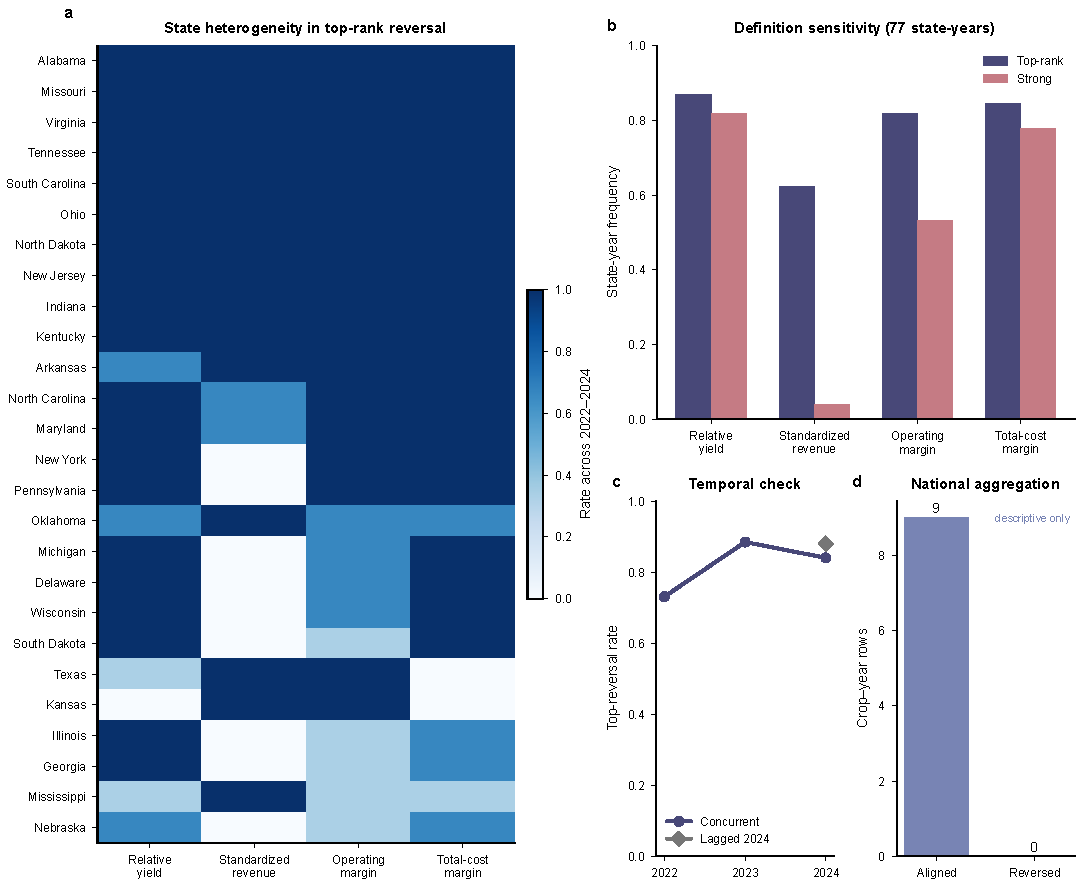
\includegraphics[width=\textwidth]{../figures/stage_ii/main/Figure6.pdf}
\caption{\textbf{Admitted-data heterogeneity and aggregation boundary.} Evidence covers \NStateYears{} state-years in \NStates{} states (\EmpiricalStartYear--\EmpiricalEndYear). Across 51 transitions per definition, every 95\% state-cluster interval for the prior-score-top versus other-crop mean share change includes zero. Concurrent inversion intensity varies by definition, state, year and national aggregation. Relative yield is nationally tied. No private-objective, constraint, CVaR, copula, causal, welfare or optimal-acreage inference is made.}
\label{fig:empirical}
\end{figure}
\clearpage
